Making computation per vertex (e.g. \textit{Flat Shading}) is more efficient because in general, a model has fewer vertices than triangles (see Table \ref{table:model-table-vertices}).
For example, the armadillo model has $15002$ vertices and $30000$ triangles, then make calculation per vertex instead of triangle results in half of the computations.

\begin{table}[!h]
    \centering
\begin{tabular}{l*{6}{c}r}
    \centering
    Model              & \#vertices & \#triangles \\
    \hline
    Armadillo          & 15002 & 30000 \\
    Eight              & 766 & 1536 \\
    Genus3             & 6652 & 13312  \\
    Horse              & 48485 &  96966\\
    Icosahedron\_1      &  42 & 80 \\
    Icosahedron\_2      &  162 & 320 \\
    Icosahedron\_3      & 642 &  1280
\end{tabular}
\caption{Comparative table: number of vertices and triangles in models.}
\label{table:model-table-vertices}
\end{table}

Making computation per edge would also be more efficient, because edges are shared between $2$ triangles in a mesh.

\subsection{Application Software}
I have developed an application for alternative data visualization using the power of barycentric coordinates and GPU programming.
\begin{figure}[!h]
    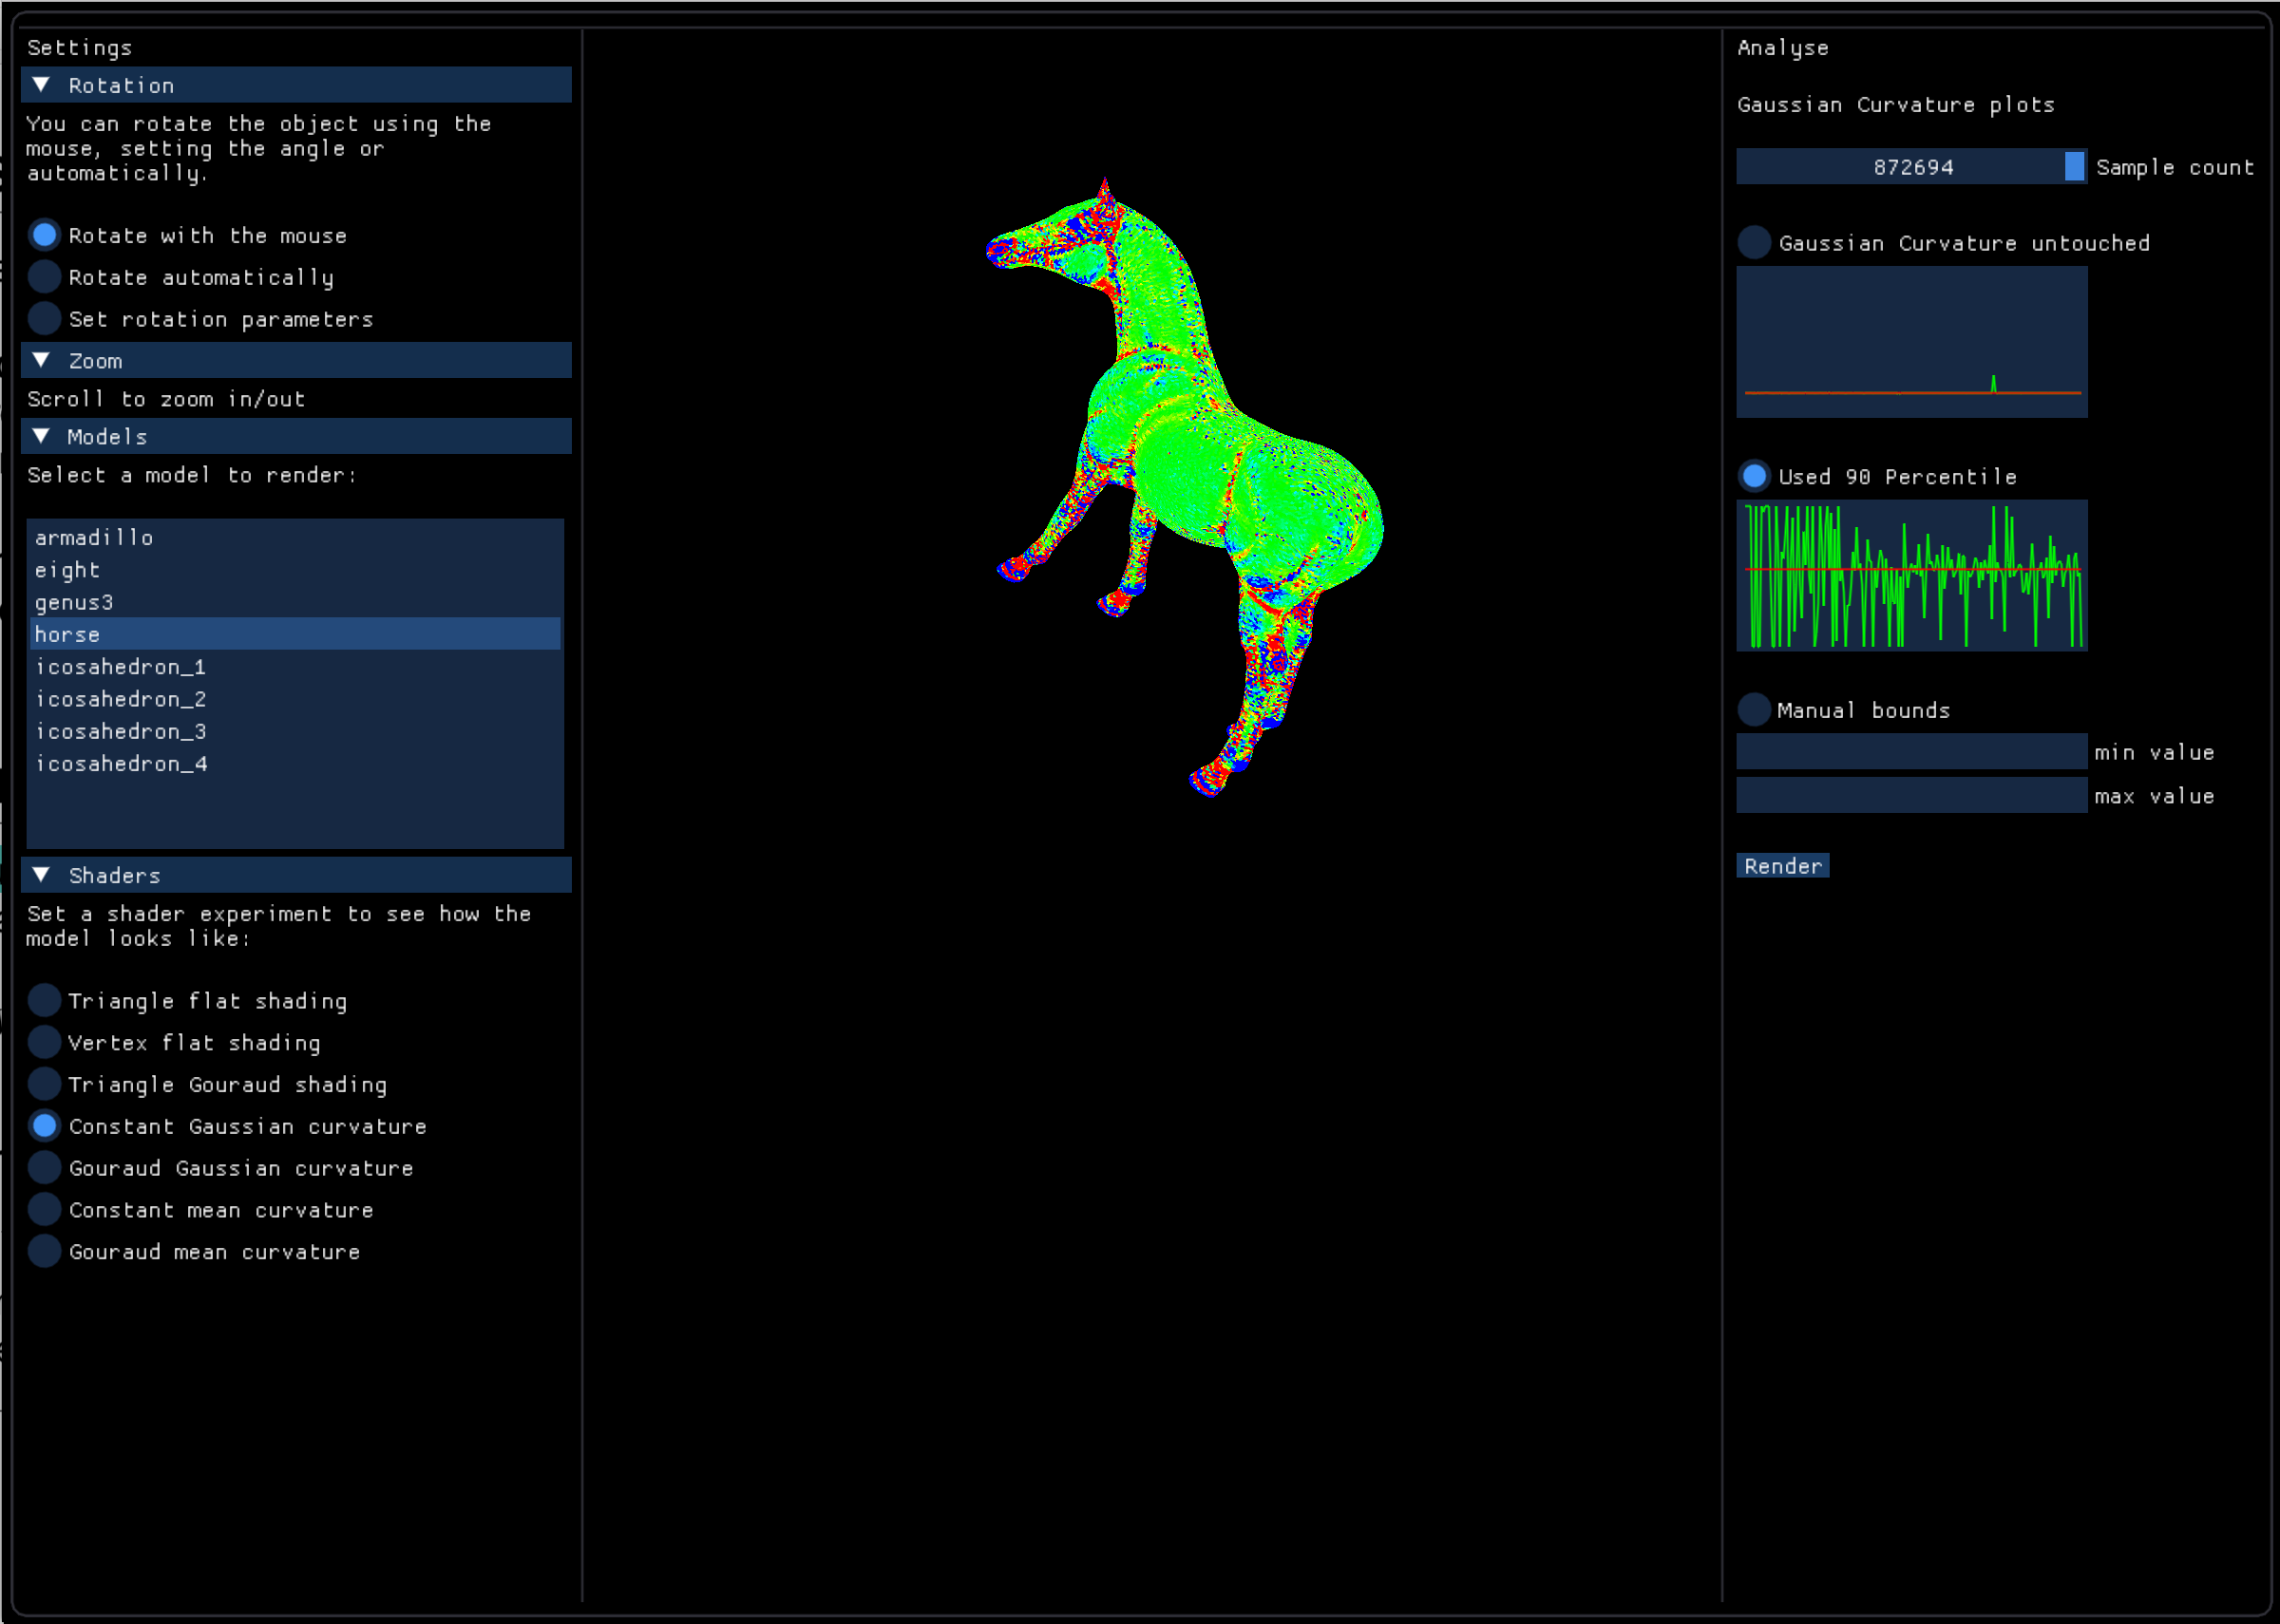
\includegraphics[scale=0.4]{images/program.png}
    \caption{Software}
    \label{fig:software}
\end{figure}
This application allows the user to upload different models, choose different shaders, zoom or rotate the model.
On Fig. \ref{fig:software}, a \textit{constant Gaussian curvature} shader is set on a model using a $90 \; percentile$, on the right graphs plot Gaussian curvature values obtained for each vertex. The first graph shows the real values of Gaussian curvature without removing the outliers. The second graph shows just the values in the $90 \; percentile$ (all the outliers were discarded).

\subsection{Architecture}
The application was developed in c++, for the real-time graphics programming (e.g. create the scene viewer, enabling the manipulation of 3D scenes) I have used OpenGL $3.3$ and GLSL.

As graphical user interface I have used a library called \textit{Dear ImGui}. This library has no external dependencies and it is designed to create content creation tools and visualization/debug tools. It is suited to integration in games engine (for tooling), real-time 3D applications or any applications on consoles platforms where operating system features are non-standard.

To allow the creation of an OpenGL context, the definition of window parameters and to handle user inputs I have used the \textit{GLFW3} library.

Since there are different versions of OpenGL drivers, to retrieve the location of the functions required and to store them in function pointers for later use, I have used \textit{GLAD} library that loads all relevant OpenGL functions according to that version at compile-time.

\subsection{Comparison with meshlab}
All the values obtained for the \textit{Gouraud Gaussian curvature} and \textit{Gouraud mean curvature} were compared to the results provided by the program \textit{meshlab}\footnote{Meshlab is an open source system for processing and editing 3D triangular meshes.
It provides a set of tools for editing, cleaning, healing, inspecting, rendering, texturing and converting meshes. It offers features for processing raw data produced by 3D digitization tools/devices and for preparing models for 3D printing. \url{http://www.meshlab.net/}}.


\begin{table}[!h]%gauss
    \centering
\begin{tabular}{l*{6}{c}r}
    \centering
    Model              & our software &  meshlab \\
    \hline
    Armadillo          & [-33034.2, 90017.9] & [-33033.843750, 90019.632812] \\
    Eight              & [-116.89, 58.3357] & [-116.889397, 58.335678] \\
    Genus3             & [-1753.2, 209.183] & [-1753.197632, 209.180344]  \\
    Horse              & [-321731, 1.93041e+06] &  [-4177.138184, 4853.229004]\\
    Icosahedron\_1      &  [1.06991, 1.07979] & [1.069908, 1.079790] \\
    Icosahedron\_2      &  [1.01461, 1.02012] & [1.014615, 1.020121] \\
    Icosahedron\_3      & [1.00291, 1.00519] &  [1.002954, 1.005204]
\end{tabular}
\caption{Comparative table: our Gouraud Gaussian curvature values ([min, max]) and meshlab Gouraud Gaussian curvature values ([min, max])}
\label{table:table-gaussian-meshlab}
\end{table}



\begin{table}[!h]%mean
    \centering
\begin{tabular}{l*{6}{c}r}
    \centering
    Model              & our software &  meshlab \\
    \hline
    Armadillo          & [-289.74, 392.54] & [-289.739105, 392.536896] \\
    Eight              & [1.34736, 10.9581] & [1.347356, 10.958117] \\
    Genus3             & [-7.02334, 117.345] & [-7.023277, 117.344765]  \\
    Horse              & [-500.961, 1202.51] &  [-500.956573, 1202.507446]\\
    Icosahedron\_1      &  [0.999998, 1] & [0.999998, 1.000002] \\
    Icosahedron\_2      &  [0.999989, 1.00009] & [0.999989, 1.000094] \\
    Icosahedron\_3      & [0.99993, 1.00007] &  [0.999930, 1.000075]
\end{tabular}
\caption{Comparative table: our Gouraud mean curvature values ([min, max]) and meshlab Gouraud mean curvature values ([min, max])}
\label{table:table-mean-meshlab}
\end{table}


